\addcontentsline{toc}{subsection}{Curve Sketching}
\subsection*{Curve Sketching}

\begin{tcolorbox}[colframe=black,sharp corners,colback=white,boxrule=.25mm]
    \begin{center}
        \textbf{Summary for Graphing Functions}
    \end{center}
    
    \vspace{.7cm}
    
    \begin{questions}
        \question Use pre-calculus and algebra
        \begin{parts}
            \part know the general shape
            \part find the $y$-intercept $(x=0)$
            \part find the roots/zeros $(y=0)$
            \part determine the vertical asymptotes (denom=0) and limits
            \part determine the horizontal or slant asymptotes
            \part use limits $x\to\pm\infty$ to determine end behavior
        \end{parts}
        
        \question Use the first derivative
        \begin{parts}
            \part determine the critical points
            \part make a first derivative sign chart to see where function is increasing or decreasing
            \part apply first derivative test to determine extrema
        \end{parts}
        
        \question Use the second derivative
        \begin{parts}
            \part determine possible points of inflection
            \part apply the second derivative test to determine extrema
            \part make a sign chart to determine concavity
        \end{parts}
    \end{questions}
    
\end{tcolorbox}

\newpage
\begin{minipage}[t]{.65\linewidth}
    \begin{center}
        \textbf{Example 1:} $y=x^3-3x^2+4$
    \end{center}
    
    \vspace{.3cm}
    
    \begin{questions}
        \question The first derivative is
        \vspace{.15cm}
        
        \question The second derivative is
        \vspace{.15cm}
        
        \question The function is increasing on
        \vspace{.15cm}
        
        \question The function is decreasing on
        \vspace{.15cm}
        
        \question The function is concave up on
        \vspace{.15cm}
        
        \question The function is concave down on
        \vspace{.15cm}
        
        \question The absolute maximum is
        \vspace{.15cm}
        
        \question The absolute minimum is
        \vspace{.15cm}
        
        \question The local maximum(s) is(are)
        \vspace{.15cm}
        
        \question The local minimums(s) is(are)
        \vspace{.15cm}
        
        \question The point(s) of inflection is(are)
    \end{questions}
\end{minipage}
\hfill
\begin{minipage}[t]{.25\linewidth}
    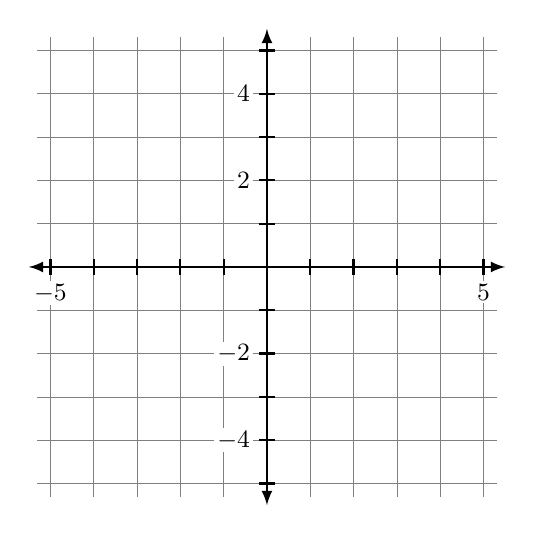
\begin{tikzpicture}[xscale=.55,yscale=.55,baseline=(current bounding box.north)]
        \draw[step=1,style=help lines,] (-5.3,-5.3) grid (5.3,5.3);
        \draw[latex-latex, thick] (-5.5,0)--(5.5,0);
        \draw[latex-latex, thick] (0,-5.5)--(0,5.5);
        \foreach \x in {-5,5}
            \draw[thick] (\x,5pt) -- (\x,-5pt) node [below=.7mm,fill=white,inner sep=1pt] {\small$\x$};
        \foreach \y in {-2,2,-4,4}
            \draw[thick] (5pt,\y) -- (-5pt,\y) node [left=.7mm,fill=white,inner sep=1pt] {\small$\y$};
        \foreach \x in {-3,-1,1,3,2,-2,4,-4}
            \draw[thick] (\x,5pt) -- (\x,-5pt);
        \foreach \y in {1,-1,3,-3,5,-5}
            \draw[thick] (5pt,\y) -- (-5pt,\y);
    \end{tikzpicture}
    
\end{minipage}

\vspace{\stretch{1}}


\begin{minipage}[t]{.65\linewidth}
    \begin{center}
        \textbf{Example 2:} $\displaystyle y=\frac{5}{2x-4}$
    \end{center}
    
    \vspace{.3cm}
    
    \begin{questions}
        \question The first derivative is
        \vspace{.15cm}
        
        \question The second derivative is
        \vspace{.15cm}
        
        \question The function is increasing on
        \vspace{.15cm}
        
        \question The function is decreasing on
        \vspace{.15cm}
        
        \question The function is concave up on
        \vspace{.15cm}
        
        \question The function is concave down on
        \vspace{.15cm}
        
        \question The absolute maximum is
        \vspace{.15cm}
        
        \question The absolute minimum is
        \vspace{.15cm}
        
        \question The local maximum(s) is(are)
        \vspace{.15cm}
        
        \question The local minimums(s) is(are)
        \vspace{.15cm}
        
        \question The point(s) of inflection is(are)
    \end{questions}
\end{minipage}
\hfill
\begin{minipage}[t]{.25\linewidth}
    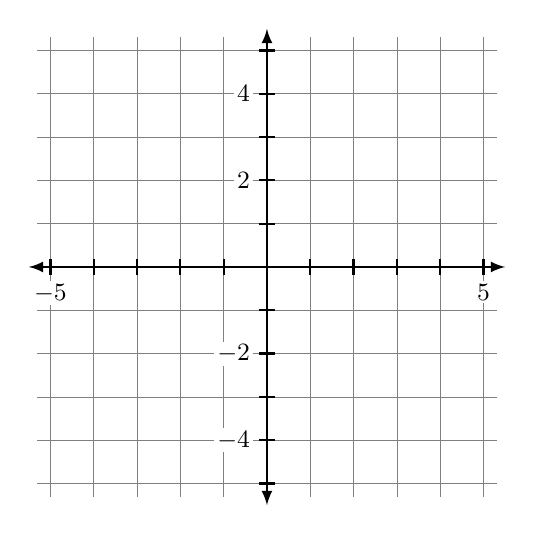
\begin{tikzpicture}[xscale=.55,yscale=.55,baseline=(current bounding box.north)]
        \draw[step=1,style=help lines,] (-5.3,-5.3) grid (5.3,5.3);
        \draw[latex-latex, thick] (-5.5,0)--(5.5,0);
        \draw[latex-latex, thick] (0,-5.5)--(0,5.5);
        \foreach \x in {-5,5}
            \draw[thick] (\x,5pt) -- (\x,-5pt) node [below=.7mm,fill=white,inner sep=1pt] {\small$\x$};
        \foreach \y in {-2,2,-4,4}
            \draw[thick] (5pt,\y) -- (-5pt,\y) node [left=.7mm,fill=white,inner sep=1pt] {\small$\y$};
        \foreach \x in {-3,-1,1,3,2,-2,4,-4}
            \draw[thick] (\x,5pt) -- (\x,-5pt);
        \foreach \y in {1,-1,3,-3,5,-5}
            \draw[thick] (5pt,\y) -- (-5pt,\y);
    \end{tikzpicture}
    
\end{minipage}

\vspace{\stretch{1}}

\newpage

\begin{minipage}[t]{.65\linewidth}
    \begin{center}
        \textbf{Example 3:} $\displaystyle y=\frac{x^2}{x^2-1}$
    \end{center}
    
    \vspace{.3cm}
    
    \begin{questions}
        \question The first derivative is
        \vspace{.15cm}
        
        \question The second derivative is
        \vspace{.15cm}
        
        \question The function is increasing on
        \vspace{.15cm}
        
        \question The function is decreasing on
        \vspace{.15cm}
        
        \question The function is concave up on
        \vspace{.15cm}
        
        \question The function is concave down on
        \vspace{.15cm}
        
        \question The absolute maximum is
        \vspace{.15cm}
        
        \question The absolute minimum is
        \vspace{.15cm}
        
        \question The local maximum(s) is(are)
        \vspace{.15cm}
        
        \question The local minimums(s) is(are)
        \vspace{.15cm}
        
        \question The point(s) of inflection is(are)
    \end{questions}
\end{minipage}
\hfill
\begin{minipage}[t]{.25\linewidth}
    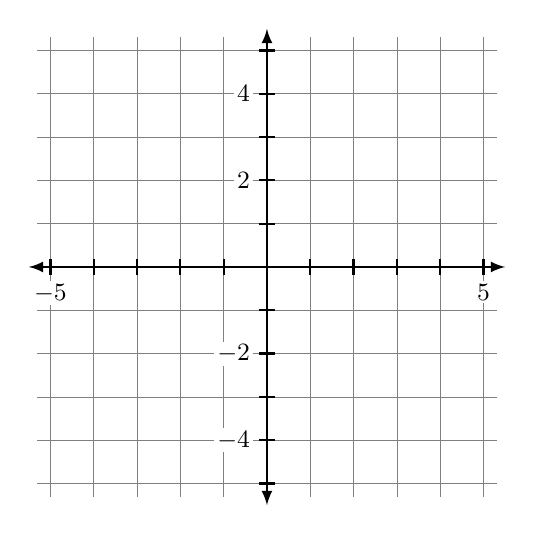
\begin{tikzpicture}[xscale=.55,yscale=.55,baseline=(current bounding box.north)]
        \draw[step=1,style=help lines,] (-5.3,-5.3) grid (5.3,5.3);
        \draw[latex-latex, thick] (-5.5,0)--(5.5,0);
        \draw[latex-latex, thick] (0,-5.5)--(0,5.5);
        \foreach \x in {-5,5}
            \draw[thick] (\x,5pt) -- (\x,-5pt) node [below=.7mm,fill=white,inner sep=1pt] {\small$\x$};
        \foreach \y in {-2,2,-4,4}
            \draw[thick] (5pt,\y) -- (-5pt,\y) node [left=.7mm,fill=white,inner sep=1pt] {\small$\y$};
        \foreach \x in {-3,-1,1,3,2,-2,4,-4}
            \draw[thick] (\x,5pt) -- (\x,-5pt);
        \foreach \y in {1,-1,3,-3,5,-5}
            \draw[thick] (5pt,\y) -- (-5pt,\y);
    \end{tikzpicture}
    
\end{minipage}

\vspace{\stretch{1}}


\begin{minipage}[t]{.65\linewidth}
    \begin{center}
        \textbf{Example 4:} $\displaystyle y=\frac{x^2+x-2}{x-2}$
    \end{center}
    
    \vspace{.3cm}
    
    \begin{questions}
        \question The first derivative is
        \vspace{.15cm}
        
        \question The second derivative is
        \vspace{.15cm}
        
        \question The function is increasing on
        \vspace{.15cm}
        
        \question The function is decreasing on
        \vspace{.15cm}
        
        \question The function is concave up on
        \vspace{.15cm}
        
        \question The function is concave down on
        \vspace{.15cm}
        
        \question The absolute maximum is
        \vspace{.15cm}
        
        \question The absolute minimum is
        \vspace{.15cm}
        
        \question The local maximum(s) is(are)
        \vspace{.15cm}
        
        \question The local minimums(s) is(are)
        \vspace{.15cm}
        
        \question The point(s) of inflection is(are)
    \end{questions}
\end{minipage}
\hfill
\begin{minipage}[t]{.25\linewidth}
    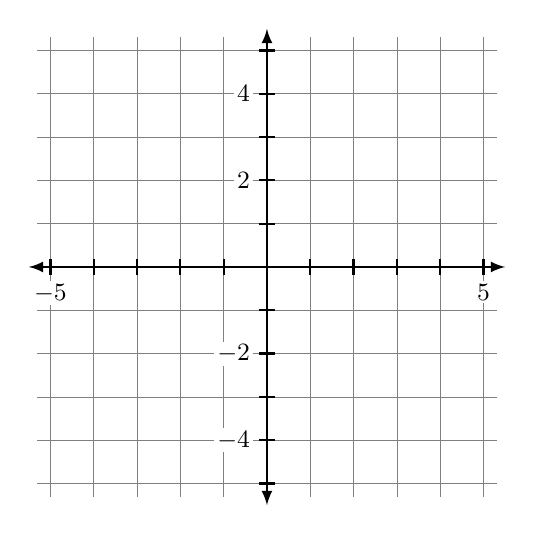
\begin{tikzpicture}[xscale=.55,yscale=.55,baseline=(current bounding box.north)]
        \draw[step=1,style=help lines,] (-5.3,-5.3) grid (5.3,5.3);
        \draw[latex-latex, thick] (-5.5,0)--(5.5,0);
        \draw[latex-latex, thick] (0,-5.5)--(0,5.5);
        \foreach \x in {-5,5}
            \draw[thick] (\x,5pt) -- (\x,-5pt) node [below=.7mm,fill=white,inner sep=1pt] {\small$\x$};
        \foreach \y in {-2,2,-4,4}
            \draw[thick] (5pt,\y) -- (-5pt,\y) node [left=.7mm,fill=white,inner sep=1pt] {\small$\y$};
        \foreach \x in {-3,-1,1,3,2,-2,4,-4}
            \draw[thick] (\x,5pt) -- (\x,-5pt);
        \foreach \y in {1,-1,3,-3,5,-5}
            \draw[thick] (5pt,\y) -- (-5pt,\y);
    \end{tikzpicture}
    
\end{minipage}

\vspace{\stretch{1}}


\newpage
